\documentclass[border=1pt,1pt]{standalone}
\usepackage{tikz}
\usetikzlibrary{arrows, decorations.markings}
\usetikzlibrary{arrows}
\usepackage{transparent}

\tikzstyle{vecArrow} = [thick, decoration={markings,mark=at position
	1 with {\arrow[semithick]{open triangle 60}}},
double distance=1.4pt, shorten >= 5.5pt,
preaction = {decorate},
postaction = {draw,line width=1.4pt, white,shorten >= 4.5pt}]
\tikzstyle{innerWhite} = [semithick, white,line width=1.4pt, shorten >= 4.5pt]

\begin{document}
\begin{tikzpicture}
\node[inner sep=0pt] (pin) at (0,0)
{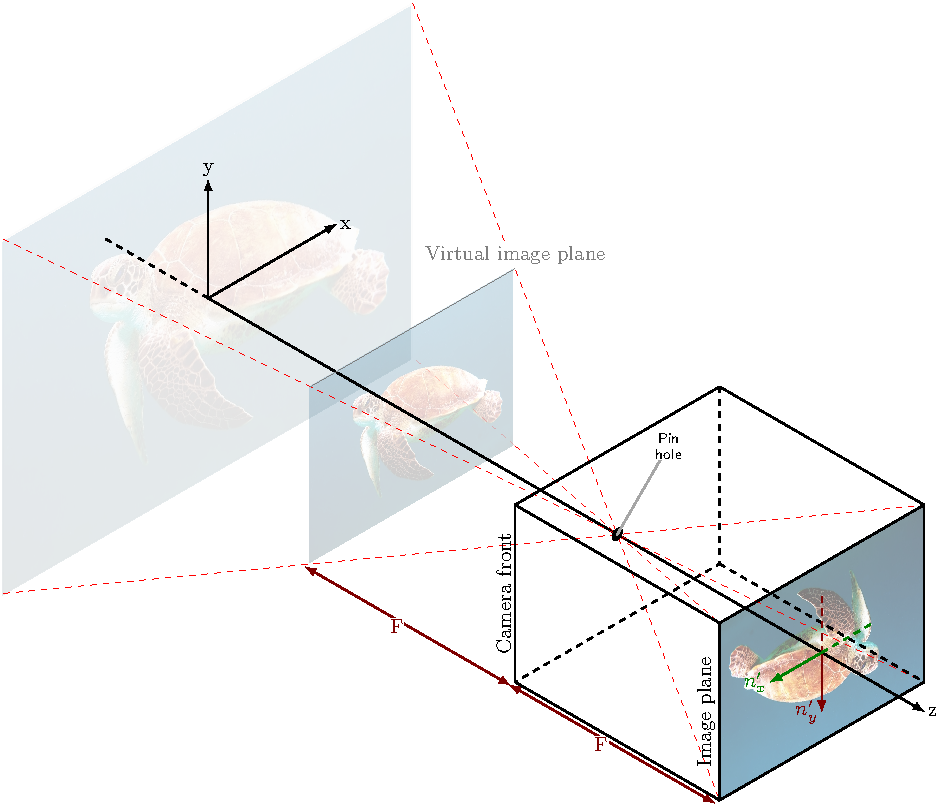
\includegraphics[]{Camera2.pdf}};
\node[inner sep=0pt] (pin2) at (17,2)
{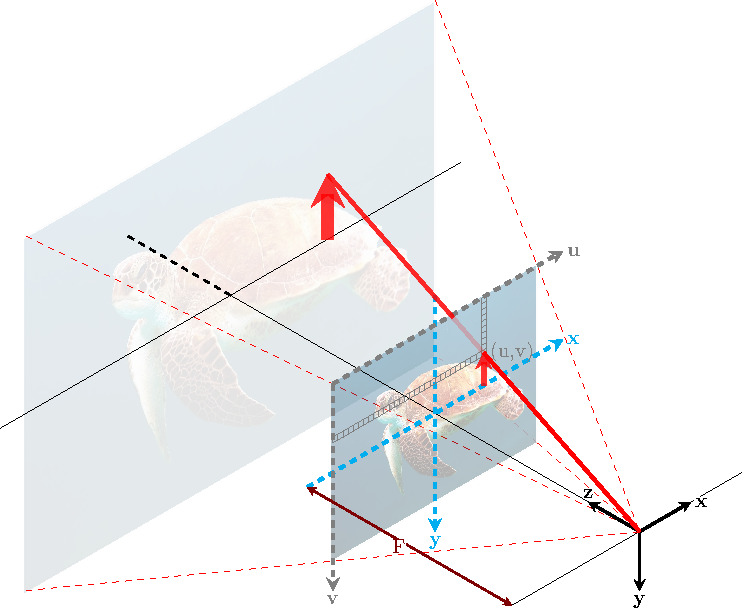
\includegraphics[]{camera3.pdf}};

\draw[vecArrow,thick] (8,1) to (10,1);
\end{tikzpicture}
\end{document}